\documentclass[../Main.tex]{subfiles}
\begin{document}
\chapter{Clean Architecture - A Craftsman's Guide  to Software Structure and Design}

\intro{
    Robert C. Martin
    ISBN-13:	978-0-13-449416-6
    ISBN-10:	0-13-449416-4
}

\section{Comparison}


Requirements:
\begin{itemize}
    \item The most important contents from the book
    \item A personal reflection about the book by the author of the summary 
    \item Regular meetings with progress and insights
    \item Atleast 3 meetings
    \item Presentations / slides of the books read by your team. In your final team-meeting, every team
    member must present his/her book using these slides. 
    \item Any proof that at least three team-sessions took place, e.g. meeting notes, video recordings, etc. 
\end{itemize}

\section{Introduction}

the	rules	of	software	architecture	are
independent	of	every	other	variable.
Wether it is a small or complex system. page 21

Difference between architecture and design -> none at all page 29
The	low-level	details	and	the	high-level
structure	are	all	part	of	the	same	whole.	

\defn{Goal}{
    The	goal	of	software	architecture	is	to	minimize	the	human	resources	required	to	build	and
 maintain	the	required	system
}

\begin{figure}[H]
    \centering
    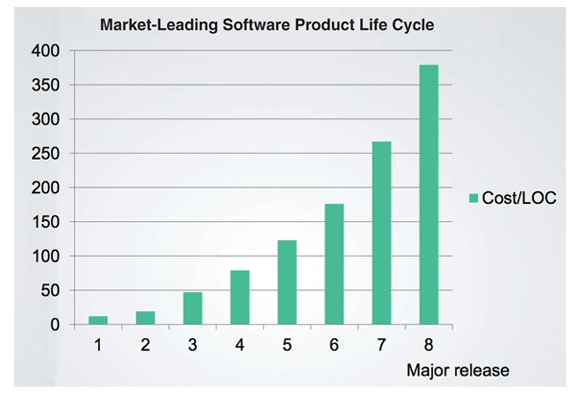
\includegraphics[width=0.75\linewidth]{Images/cpl-over-time.png}
    \caption{Cost per line increases over time due to complexity. More staff is required. This business model in insustainable}
\end{figure}

\begin{itemize}
    \item Take quality seriously. Don't "change later".
\end{itemize}

\section{Values}
Software provides two values:
\begin{description}
    \item[Behavior] How the software meets stakeholder requirements.
    [Structure] how easily the software can be changed.
\end{description}

Developers ensure both behavior and structure are high.

\begin{description}
    \item[Behavior]
    Developers make machines behave according to requirements.
    Debugging and fixing issues when the behavior deviates.
    Structure:
    [Software] must be "soft" and easy to change.
    Changes should only depend on scope, not the system's complexity.
    Over time, changes get harder if the system's architecture isn't flexible.
    [Architecture]
    Needs to be shape-agnostic to allow easy integration of new features.
    Should not prefer one shape over another, to avoid complex fitting of new features.
\end{description}

Key-Take-Away:
\begin{itemize}
    \item A system with poor architecture can lead to high costs for future changes,
    making it more important for software to be easy to modify than to be initially functional without flexibility.
    \item Focus on both, not just one.
\end{itemize}

\section{Paradigms}

\defn{Structured}{
    Structured	programming	imposes	discipline	on	direct	transfer	of	control.
    When dismissing goto statements one could proof programs.
    \begin{itemize}
        \item Proofable Programs is not widely used.
        \item Tests use the "scientific" not the matematical method.
        It proofs something is not wrong, not that something is correct.
        \item Software that is not provable (goto) cannot be deemed correct.
        \item modern	languages	do	not
        typically	support	unrestrained	goto	statements.
    \end{itemize}
    Structured	programming	forces	us	to	recursively	decompose	a	program	into	a	set
    of	small	provable	functions.	We	can	then	use	tests	to	try	to	prove	those	small
    provable	functions	incorrect.	If	such	tests	fail	to	prove	incorrectness,	then	we
    deem	the	functions	to	be	correct	enough	for	our	purposes.
   
}

\defn{Object Oriented}{
    Object-oriented	programming	imposes	discipline	on	indirect	transfer	of	control.
    \textit{encapsulation,	inheritance,	and	polymorphism}

    OO	is	the	ability,	through	the
    use	of	polymorphism,	to	gain	absolute	control	over	every	source	code
    dependency	in	the	system.	It	allows	the	architect	to	create	a	plugin	architecture,
    in	which	modules	that	contain	high-level	policies	are	independent	of	modules
    that	contain	low-level	details.	The	low-level	details	are	relegated	to	plugin
    modules	that	can	be	deployed	and	developed	independently	from	the	modules
    that	contain	high-level	policies
}

\defn{Funcational}{
    Functional	programming	imposes	discipline	upon	assignment.
    TBD
    e.g paralellize!!!!
}

Each	of	the	paradigms	removes	capabilities	from	the
programmer.

Aims of a software architect:
\begin{itemize}
    \item Software	architects	strive
    to	define	modules,	components,	and	services	that	are	easily	falsifiable	(testable).
    \ item 
\end{itemize}

\end{document}
